\documentclass{amsart}
\usepackage[utf8]{inputenc}
\usepackage{graphicx}
\usepackage{enumerate}
\usepackage{comment}
\usepackage{multirow}
\usepackage[a4paper]{geometry}
\geometry{ a4paper, left = 1cm, right = 1cm, top = 1cm, bottom = 1cm}

\begin{document}
    \hrule
    \begin{center}
        \textbf{ Lamma    Tommaso    0000881007        Turno    IV }
    \end{center}
    \hrule
    \begin{center}
        {\huge Misura della caratteristica di due diodi a giunzione p-n}
    \end{center}
    Lo scopo della prova era la misura della caratteristica di un diodo al Silicio ed uno al Germanio
    per ricavare il parametro $\eta V_T$ della legge di Schottky, preceduta dalla calibrazione di oscilloscopio e 
    multimetro digitale.\\
    Il circuito utilizzato per la prova è il seguente :
    \begin{center}
        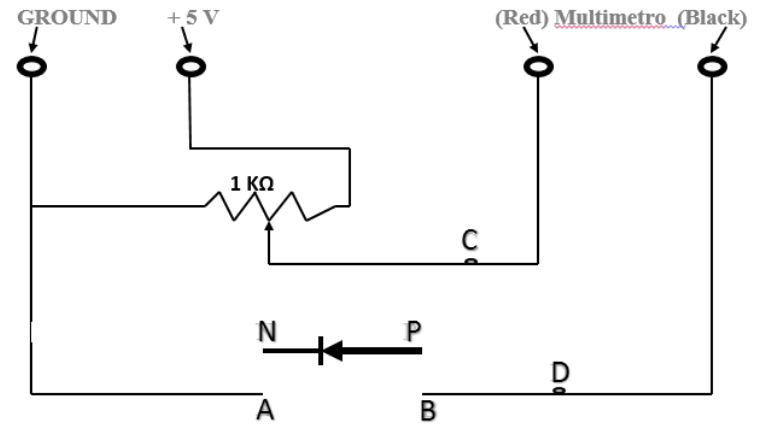
\includegraphics[width = 10cm, height = 7cm]{circuito.png}.
    \end{center}
    Gli strumenti utilizzati nella prova sono:
    \begin{enumerate}[(i)]
        \item Potenziometro da 1$k\Omega$
        \item Diodi a giunzione p-n: AAZ15/OA47 Germanio, 1N914A/1N4446/1N4148 Silicio
        \item Breadboard generica
        \item Oscilloscopio ISR 622 ISO-TECH
        \item Multimetro digitale FLUKE 75
        \item Generatore di tensione continua IPS 3303 ISO-TECH
    \end{enumerate}
    I dati misurati per la calibrazione di multimetro ed oscilloscopio, per la caratteristica del diodo al Silicio 
    e di quello al Germanio sono rispettivamente, utilizzando un fondoscala fisso per i diodi di $0.1V$:\\
    \hfill \\
    \begin{center}
        \begin{tabular}{|p{2cm}|p{2cm}|p{2cm}|p{2cm}|p{2cm}|}
            \hline
            \multicolumn{5}{|c|}{Calibrazione}\\
            \hline
            $V_{mul}$[V] & $\delta V_{mul}$[V] & $V_{osc}$[V] & $\delta V_{osc}$[V] & fondoscala[V]\\
            \hline
            0.099 & 0.0003 & 0.1 & 0.002 & 0.02\\
            0.151 & 0.0004 & 0.15 & 0.005 & 0.05\\
            0.199 & 0.0005 & 0.2 & 0.005 & 0.05\\
            0.294 & 0.0006 & 0.3 & 0.01 & 0.1\\
            0.394 & 0.0008 & 0.4 & 0.01 & 0.1\\
            0.491 & 0.0009 & 0.5 & 0.01 & 0.1\\
            0.591 & 0.001 & 0.6 & 0.01 & 0.1\\
            0.691 & 0.003 & 0.7 & 0.02 & 0.2\\
            0.791 & 0.003 & 0.8 & 0.02 & 0.2\\
            \hline
        \end{tabular}\\
        \vspace{0.2cm}
        \begin{tabular}{|p{1cm}|p{1cm}|p{1cm}|p{1cm}|}
            \hline
            \multicolumn{4}{|c|}{Silicio}\\
            \hline
            \textbf V[V] & $\delta$V[V] & I[mA] & $\delta$I[mA] \\
            \hline
            0.07 & 0.01 & 0.01 & 0.0004\\
            0.08 & 0.01 & 0.01 & 0.0004\\
            0.1  & 0.01 & 0.02 & 0.0005\\
            0.12 & 0.01 & 0.04 & 0.0007\\
            0.14 & 0.01 & 0.07 & 0.001\\
            0.16 & 0.01 & 0.10 & 0.004\\
            0.18 & 0.01 & 0.16 & 0.005\\
            0.20 & 0.01 & 0.24 & 0.005\\
            0.24 & 0.01 & 0.53 & 0.008\\
            0.26 & 0.01 & 0.73 & 0.01\\
            0.28 & 0.01 & 1.07 & 0.04\\
            0.29 & 0.01 & 1.26 & 0.04\\
            0.30 & 0.01 & 1.48 & 0.04\\
            0.31 & 0.01 & 1.74 & 0.05\\
            0.32 & 0.01 & 2.03 & 0.05\\
            \hline      
        \end{tabular}
        \hspace{2cm}
        \begin{tabular}{|p{1cm}|p{1cm}|p{1cm}|p{1cm}|}
            \hline
            \multicolumn{4}{|c|}{Germanio}\\
            \hline
            \textbf V[V] & $\delta$V[V] & I[mA] & $\delta$I[mA] \\
            \hline
            0.4 & 0.01 & 0.01 & 0.0004\\
            0.5 & 0.01 & 0.06 & 0.0009\\
            0.54 & 0.01 & 0.12 & 0.003\\
            0.56 & 0.01 & 0.2 & 0.005\\
            0.58 & 0.01 & 0.25 & 0.006\\
            0.59 & 0.01 & 0.33 & 0.006\\
            0.6 & 0.01 & 0.42 & 0.007\\
            0.61 & 0.01 & 0.5 & 0.008\\
            0.62 & 0.01 & 0.6 & 0.009\\
            0.64 & 0.01 & 0.92 & 0.01\\
            0.65 & 0.01 & 1.06 & 0.03\\
            0.66 & 0.01 & 1.27 & 0.03\\
            0.67 & 0.01 & 1.55 & 0.05\\
            0.68 & 0.01 & 1.88 & 0.05\\
            0.7 & 0.01 & 2.65 & 0.06\\
            \hline
        \end{tabular}
    \end{center}
    I loro rispettivi grafici sono:\\
    \hfill \\
    \begin{center}
        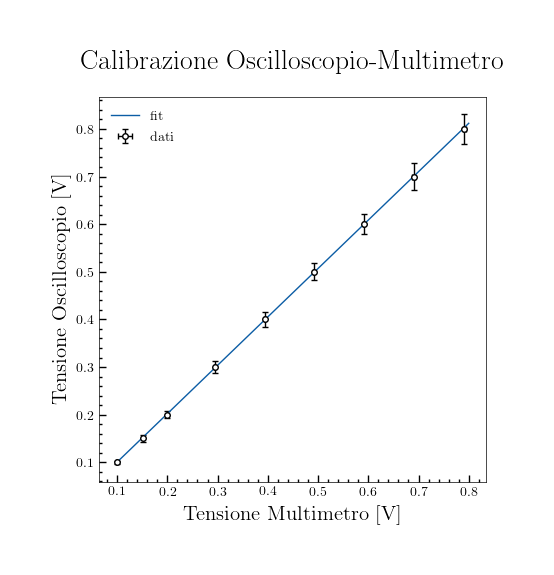
\includegraphics[width = 8cm, height = 8cm]{calibrazione/grafico_calibrazione.png}\\
        \vspace{0.5cm}
        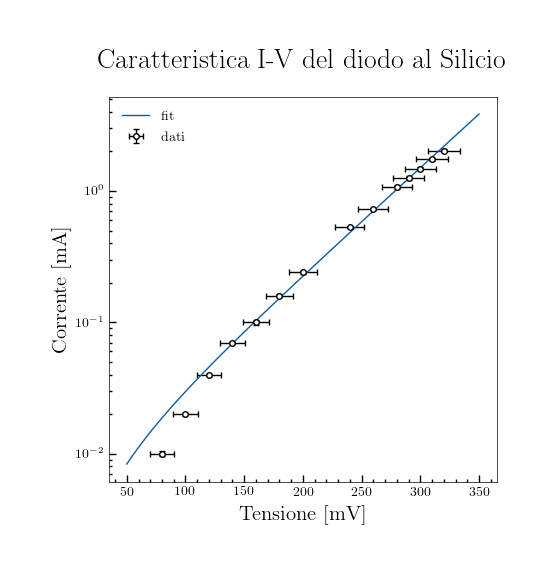
\includegraphics[width = 8cm, height = 8cm]{silicio/grafico_silicio.png}
        \hspace{0.1cm}
        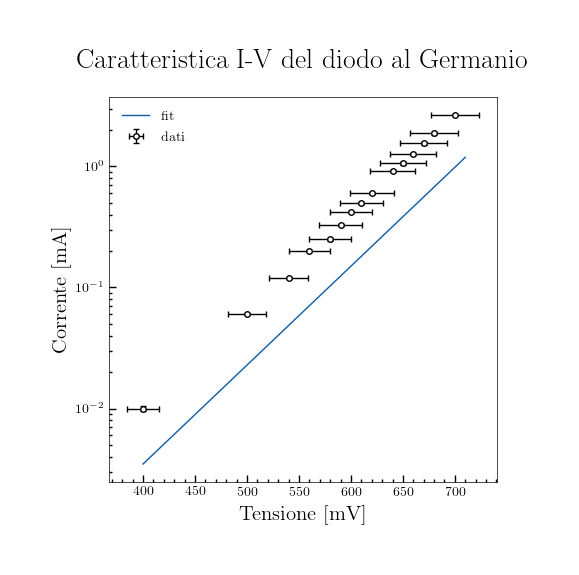
\includegraphics[width = 8cm, height = 8cm]{germanio/grafico_germanio.png}
    \end{center}
    I risultati finali sono:\\
    \hfill \\
    \begin{center}
        \begin{tabular}{|p{2cm}|p{1cm}|p{2cm}|}
            \hline
            Calibrazione & slope & $1.02 \pm 0.02$ \\
            \hline
            \multirow{2}{*}{Silicio}      & $\eta V_T$ & $(53 \pm 4)mV$ \\
                                        & $I_0$ & $0.0053 \pm $ \\
            \hline
            \multirow{2}{*}{Germanio}      & $\eta V_T$ & $(53 \pm 3)mV$ \\
                                        & $I_0$ & $ 5 \cdot 10^{-6} \pm $\\
            \hline  
        \end{tabular}
    \end{center}
    \vspace{0.5cm}
    Le stime dei parametri riportati nella precedente tabella e delle relative incertezze sono state ricavate da fit lineari pesati
    considerando soltanto gli errori sulla tensione misurata con l'oscilloscopioin quanto relativamente maggiori 
    a quelli sulla corrente o sulla tensione misurate dal multimetro, per le caratteristiche dei diodi il fit lineare è stato 
    fatto utilizzando il logaritmo delle correnti. Per la corrente $I_0$ nel caso dei diodi si sono propagate le incertezze rispetto
    ai parametri di pendenza ed intercetta restituiti dal fit. Nel caso del diodo al Silicio si è scelto di fittare solo per tensioni
    superiori ai $150mV$.
\end{document}